
\chapter{Data collection}

\section{Background on survey design}

%TODO 1 cite: https://books.google.co.uk/books?id=mSRTDwAAQBAJ&lpg=PP1&ots=nynKGurXVG&dq=how%20to%20write%20a%20survey&lr&pg=PP1#v=onepage&q&f=false
%TODO 2 cite: https://www.idsurvey.com/en/advantages-and-disadvantages-of-phone-survey/
%TODO 3 cite: https://books.google.co.uk/books?hl=en&lr=&id=ctow8zWdyFgC&oi=fnd&pg=PR15&dq=survey+methodology&ots=fgcIbBXkS9&sig=LvdOfWOBGrtHFrcVbdfi1ahV970#v=onepage&q=survey%20methodology&f=true
%TODO 4 cite: https://en.wikipedia.org/wiki/Census
%TODO 5 cite: https://www.understandingsociety.ac.uk/
%TODO 6 cite: https://ora.ox.ac.uk/objects/uuid:526114c2-8266-4dee-b663-351119249fd5
%TODO 7 cite: https://www.nature.com/articles/bdj.2008.149
%TODO 8 cite: https://www.collinsdictionary.com/dictionary/english/systematic



As explained in [CITE 3 HERE], a survey is a means of obtaining quantitative information regarding opinions and 
experiences of the respondents in order to explore the views of the target population as a whole. In this book, a survey 
is noted as a ``systematic" method of collecting data, where the author states that the word ``systematic" is deliberately used 
in order to separate surveys from other methods of information collection. The word ``systematic'' is defined by the Collins English Dictionary as 
something that \textit{"is done according to a fixed plan, in a thorough and efficient way"} [CITE 8 HERE], and this reflects that a survey is 
highly structured, with each participant being asked to answer standardised set of questions with no deviation from the 'fixed plan' of the
survey. However, while having a 'fixed plan' is a key defining factor of a survey, whether or not the survey is 'thorough' and
'efficient' depends heavily on the survey structure and design. Designing an effective, systematic survey involves the task of balancing 
being thorough alongside being efficient, and this will be discussed in more depth later. A survey of a systematic nature as described here has the 
ability to yield a large volume of easily comparable results as every participant has been asked the same exact questions.


This is in contrast to the more free-form structure of focus groups and unstructured or semi-structured interviews. These are less systematic as they 
involve back-and-forth discussion between the participants and interviewer, which is discussed in 

can be more difficult to 
analyse statistically, and are better suited for gaining 
general insights rather than to undergo rigorous statistical testing. 


As mentioned above, survey methodology involves asking a sample of the target population a series of standardised questions, 
which may be presented in mediums such as written questionaires or structured interviews. Depending on the aims of the study, there
will be many benefits and downfalls of each method. There may also be times when a combined approach is required to
gather the necessary information.

Phone calls and other forms of interview-based survey allow the interviewer to form a personal connection with 
the survey participant, which can be especially helpful for a company's image if the interviewer is particularly professional 
or charismatic. Additionally, while the interviewer will still be limited to asking the pre-set questions, the format of such a survey can 
be considered semi-structured and with much more room for interpretation. This can lend itself to gaining additional insights
that may not have otherwise been gathered from a more closed-form paper or online survey. Additionally, the more open format
can negate any error as a result of participants misinterpreting questions due to the interviewer's ability to immediately 
clarify on any misunderstandings. This type of survey also provides an instant response, which is beneficial if there is only 
a short time frame available in which to gather information. 

However, there are also shortfalls to an interview-based survey method. For instance, although a charismatic interviewer can 
positively impact the image of whoever is conducting the survey, this could also lead to biases, such as the respondent 
answering in a way they feel will please the interviwer.
Additionally, the image of the organisation could potentially be tainted if the interviwer appears rude or unprofessional, 
alongside potentially providing bias in the opposite direction. As well as this, telephone surveys are likely to be 
interpreted as a telemarketing scheme, and thus potentially have a negative impact on the number of willing respondents.
The reduced anonymity of this type of survey may also create bias in the way of participants avoiding making statements
that could be deemed socially unacceptable, or that they feel they may be judged for, and therefore may not provide answers
accurate to their true line of thought.

A second way of presenting survey questions, and the way that will be used in this study, is a self-completed written questionaire.
A questionaire may either consist of physical paper forms that are mailed or handed out to people within the target population, or may
exist in an online format. As discussed in [CITE 1 HERE], this form of surveying 

A questionaire is composed of two types of questions; closed-ended questions, where participants 
select answers from a given set, and open-ended questions, in which the participants are able to provide free-form answers. 

This method of surveying
is also often anonymous, which can mitigate the errors caused by participants fearing being judged on their responses. Closed-ended questions are
very good for obtaining quantitative data as the answers may be easily categorised and counted. Open-ended questions are generally used to 

The UK Household Longitudinal Study is an ongoing study and an example of implementation of a combined use of the above mentioned surveying methods.
Initially, in 'wave 1' of the study, a sample of 40,000 households in the UK were selected to be surveyed on a yearly basis. The survey involves all 
members of each selected household, overall comprising of around 100,000 individials, and asks them a wide range of questions
%TODO Expand on this





\section{Specific goals of survey tool for this study}
While visualisations can be a very useful tool for understanding data, they also have the potential to be highly misleading. This section of the 
study will explore how modifying certain aesthetic features of visualisations can impact perception and interpretation of data, and how these 
modifications can be exploited in order to mislead the observer. Misleading visualisations may be created in an effort to deliberately influence the 
viewers' perceptions, or accidentally as a result of poor practice and knowledge surrounding data visualisation. In either case, visualisations have the
ability to communicate different messages and stories depending on how they present the data to the observer. There is a large amount of research and 
literature surrounding this topic, both in terms of providing frameworks for good visualisation practice as well as looking into how various techniques 
are used to decieve viewers. Results from some of these papers will be replicated, as well as used to form hypotheses which this survey will investigate.\newline

One feature that will be tested is scaling of axes. This is widely regarded in literature to be a commonly used tactic for misleading the observer.

 





A large amount of the literature exploring misleading tactics in data visualisation focusses mainly on bar plots and line plots for categorical and 
time series data, and so this is what the survey will also focus on. There is also a large amount of literature surrounding the use of three dimensional 
viualisations and pie charts, which will not be explored here however will be discussed in later sections. 


In particular, the results formulated in [CITE: https://dl.acm.org/doi/pdf/10.1145/3380851.3416762] will
be explored. Similarly to our study, the paper uses a survey to explore how deceptive visualisation techniques can be employed as well as their impact 
on perception of the data. The survey discussed in this paper presents the participant with four plots; a bar plot, a line plot, a pie chart and a 
bubble plot, 









The first example shows how truncating the y-axis of a bar plot can overexaggerate differences in the heights of the bars, perhaps leading to incorrect 
observations regarding comparisons of values within the data. A first hypothesis that will be tested in this survey is that truncating the y-axis
does indeed impact how the data is interpreted.

For example, if the data consists of values, such as profits, at different time points, then truncating 
the y-axis can at first make the profit increase each year seem much greater than it actually is. Only when one reads the scale on the 
axis will it be observed that there may only be a very marginal, and potentially almost negligible, difference. Of course if someone 
were to read the y-axis scaling they would determine that the change was in fact small, but the human brain thrives on visual and 
pictorial feedback, and thus it is likely that a person would look at this plot and simply draw conclusions based on the plot itself
without reference to the truncated axis.  Additionally, the use of a logarithmic scale will be investigated, and it will
be hypothesised that this will also impact interpretation.



\section{Survey Design}

Although the content of the 
surveys for this study is not likely to be controversial or highly personal, anonymity is still important as the participants could otherwise 
potentially feel pressure to give a 'correct' answer, given the mathematical nature of the questions. Anonymity here means that this pressure 
is potentially reduced and thus the relevant measurement bias may be mitigated. The questionaire will also contain 


The publication [CITE: https://dl.acm.org/doi/pdf/10.1145/3380851.3416762] was used as inspiration for survey design.

The decision to focus on the two plot types was made in part to follow the existing literature, but also to ensure the survey is not too long. 
As discussed in [CITE: https://ojs.ub.uni-konstanz.de/srm/article/view/7145], too long a survey can result in higher measurement error due to factors 
such as waning interest or mental fatigue of respondents, resulting in careless responding and non-response. This is also further explored in 
[CITE: https://corescholar.libraries.wright.edu/cgi/viewcontent.cgi?article=3059&context=etd_all]. While 
[CITE: https://ojs.ub.uni-konstanz.de/srm/article/view/7145] does conclude that a 'split survey' design, where each respondent is only asked to 
answer a selection of questions from the whole set, is effective in reducing error while gathering large amount of information, this will not be employed
here. The reasoning for this is that there will already be a large set of different surveys being sent, and creating further splits could potentially lead
to small sample sizes and thus inconclusive results. Additionally to this, the paper investigates how placement of questions in the survey can affect
responses, concluding that questions asked later in the survey are more susceptible to bias. 

%%%%% TODO:

% Perform meta-analysis of different sources to find optimal number of survey questions?
% "20 minute rule" -> Don't go beyond 20 mins
% Work out how long each question will take... Guessing 1-2 mins per question => ~10-20 questions?
% Long surveys can increase measurement error
% 

%%%%% Potential sources about survey length %%%%%
% https://journals.sagepub.com/doi/pdf/10.2501/IJMR-2017-039 -> Study about ideal length of survey in terms of time
% https://ojs.ub.uni-konstanz.de/srm/article/view/7145 -> Study about reducing measurement error due to survey length
% https://corescholar.libraries.wright.edu/etd_all/1918/ -> About 'careless responding' and 'insufficient effort responding'
% https://journals.sagepub.com/doi/abs/10.1177/089443930101900202 

Two types of questionaire will be written for this study. The first type will present a series of fairly basic visualisations accompanied
by questions created to guage whether each presented visualisation has an impact on how the data is interpreted by the survey participant.


The set will consist of three separate surveys, which will be identical up to the visualisation package used. Particularly, one will contain 
visualisations made with R's ggplot2, the next with matplotlib from Python, and the last with the JavaScript library D3. These surveys will 
be distributed to the general public by sharing links on social media platforms such as Facebook. The reasoning behind creating three separate 
surveys in a variety of languages is to ascertain whether the language used influences the interpretation. 




%TODO explain the second type of survey further
The second type will be a single survey comparing the implementation of the different languages and will be distributed to a group specialising 
in visual analytics for pharmaceutical research. This second survey aims to explore opinions on the coding languages themselves, in terms of 
features such as readability, reproducibility and ease of implementation.

%TODO explain that I'm using questionaires and why


In the set of three surveys we aim to answer questions such as: 

\begin{itemize}
    \item In which form is the given information of interest most accurately interpreted by the viewer?
    \item What factors of a plot can bias interpretation? 
    \item Does the visualisation tool used have an impact on interpretation?
    \item Does the tool used have an impact on opinions regarding aesthetic features?
\end{itemize}


% Idea: Since I have had to extract things from ninja warrior data (lots of data), could show data and then a plot to show how
%       visualisations are useful to find things you can't immediately see in the data itself.
% Idea: Axes in time series plots - Use short and tall axes and ask which varies most? (Maybe use HR data from http://ecg.mit.edu/time-series/)
% Idea: Distance between bars in barplot - further apart harder to interpret?
% Idea: Does uning a logarithmic scale impact interpretation?

\section{The survey}

Potentially will use google sheets and post all three, and ask people to complete one of them.
%TODO Specify further

\section{\textbf{Demographic Questions}}

The questions below are used to 

\begin{itemize}
    \item Please enter your age
    
    \item If you are a university student or past university graduate please specify your area of study. (Drop down box: Science, Technology, Engineering, Maths, Arts, Social Sciences, Humanities, Business, N/A, Other (please specify))

    \item How strongly do you agree with each of the following statements? (Linear scale with 1 - 5, 1=strongly disagree, 5=strongly agree)

    \item\item I have good spatial awareness skills 
    
    \item\item I have good observational skills 
    
    \item\item I have good numerical skills 
    
    \item Are you colourblind? (Checkbox: Yes, No, Prefer not to answer)
    
    \item Do you have any disorders that may affect visual processing? (this could be a general visual processing disorder 
    or dyslexia, dyscalculia etc)
    ((Checkbox: Yes, No, Prefer not to answer))
\end{itemize}


\section{\textbf{Bar Plot Questions}}

American Ninja Warrior\newline

The following bar charts present information regarding how many times 4 obstacles were used over the course of 10 seasons of the TV show 'American Ninja Warrior'. Please note that the answers to this section are entirely subjective, and that there are no 'correct' answers.\newline


The first three questions refer to this bar chart, bar chart A.

\textbf{Figure}

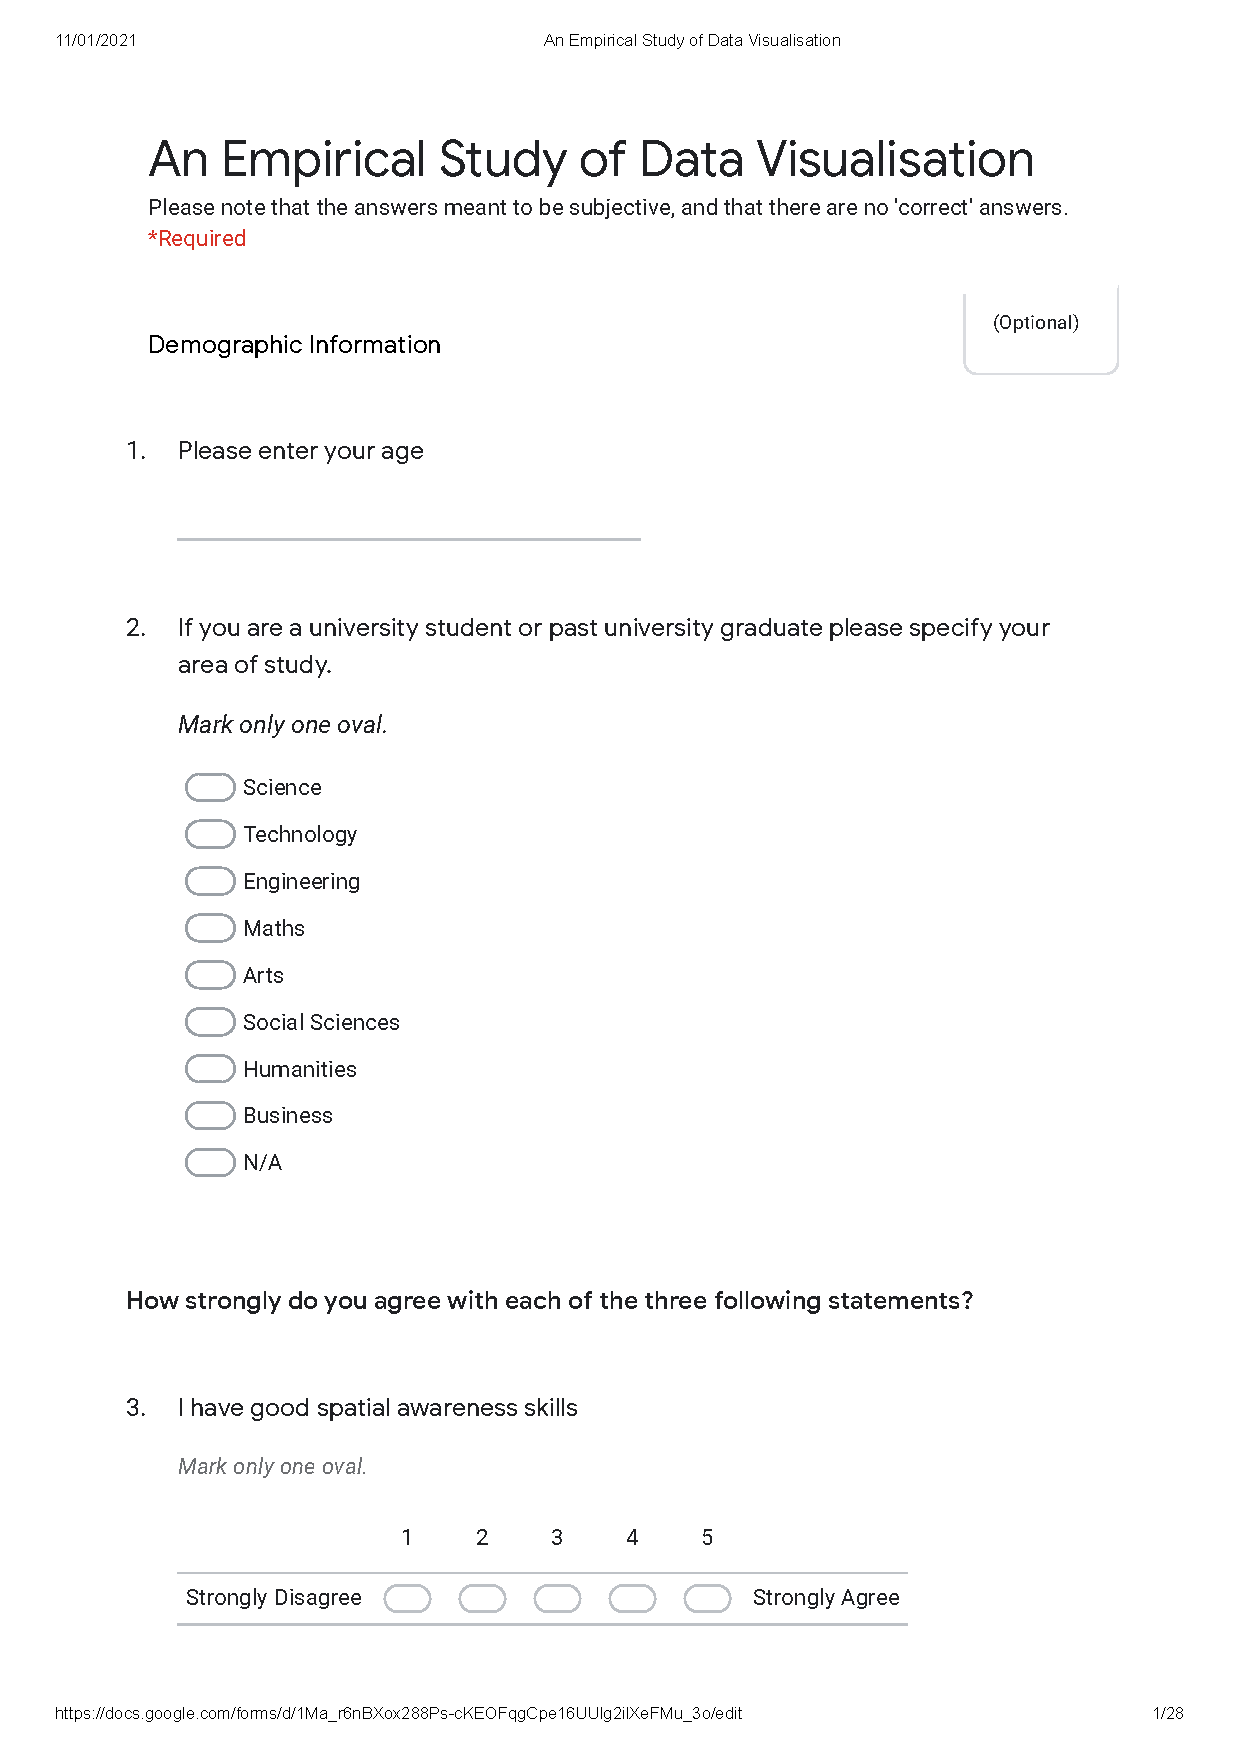
\includepdf[pages=-, pagecommand={}]{C:/Users/Katie/OneDrive/Uni_Work_Year4/Project/Year-4-Project/survey responses/An Empirical Study of Data Visualisation (R - v1) - Google Forms}



%Note: Deliberately design 'bad' as well as good plots?

%%%%% Misleading aspects of plots: %%%%%

% Axis Scales
% - Sources:
%   - https://www.nature.com/articles/s41559-018-0610-7
%   - https://web.archive.org/web/20101123050530/http://graphpad.com/faq/file/1487logaxes.pdf
%   - https://dl.acm.org/doi/fullHtml/10.1145/3231772
%   - https://journals.sagepub.com/doi/pdf/10.1177/1050651920958392 
%   - https://journals.sagepub.com/doi/pdf/10.1177/1050651920958392
%   - 


%%%%%

% TODO Write about choosing more 'basic' questions to cut down on number of questions as well as appealing to audience



\section{Conclusion}
